\documentclass[convert = false, tikz]{standalone}
\usepackage[utf8]{inputenc}
\usepackage{tikz}
\usetikzlibrary{automata, positioning, arrows}
 
\usepackage{../../../../style_automata}

% arara: pdflatex
% arara: latexmk: { clean: partial }
\begin{document}
    \tikzset{
    node distance=2cm, % specifies the minimum distance between two nodes.
    }
    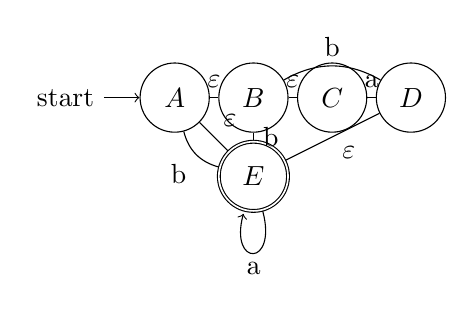
\begin{tikzpicture}
        \node[state, initial] (a) {$A$};
        \node[state, right of=a] (b) {$B$};
        \node[state, right of=b] (c) {$C$};
        \node[state, right of=c] (d) {$D$};
        \node[state, accepting, below of=b] (e) {$E$};
        \draw (a) edge[above] node{\(\varepsilon\)} (b)
        (b) edge[above] node{\(\varepsilon\)} (c)
        (c) edge[above] node{a} (d)
        (a) edge[above right] node{\(\varepsilon\)} (e)
        (b) edge[right] node{b} (e)
        (d) edge[below right] node{\(\varepsilon\)} (e)
        (e) edge[below left, bend left] node{b} (a)
        (d) edge[above, bend right] node{b} (b)
        (e) edge[loop below] node{a} (e);
    \end{tikzpicture}
\end{document}